\section{研究目标与总体技术路线回顾}

\subsection{研究背景与课题意义}

\paragraph{大规模SoC验证对执行性能与可观测性的需求}

随着片上系统（System-on-Chip，SoC）的功能和规模不断增加，芯片验证已不再局限于单个硬件模块的功能测试。处理器、存储子系统和各类外设之间的交互，还需要通过固件、操作系统以及应用程序等软件负载进行系统级验证。这类测试往往需要执行大量时钟周期，并在发现异常后检查其发生前后的硬件状态。因此，验证平台既要能够运行足够复杂的RTL设计，也要具备较高的执行效率和内部状态可观测性。

传统RTL软件仿真能够在信号级观察和调试电路行为，适合定位具体的设计错误。但当测试对象扩展为完整SoC，且需要运行操作系统或较长的软件负载时，仿真速度容易成为限制。基于FPGA的硬件仿真加速将RTL逻辑映射到可编程硬件上执行，可以显著缩短系统级负载的运行时间。FireSim等研究已展示了FPGA加速在周期精确系统仿真中的应用\cite{chung_firesim_2018}。然而，单片FPGA的逻辑、存储和互连资源有限，难以持续适应不断增长的DUT规模。

执行速度和设计容量之外，调试能力同样重要。例如，系统在运行较长时间后才出现错误时，验证人员不仅需要知道程序在哪里失败，还可能需要观察错误发生前数千个周期的寄存器、存储器及控制信号。传统FPGA原型验证可以借助片上逻辑分析和波形捕获进行调试，但可观测信号、存储深度以及触发时机通常受到硬件资源和预先配置的限制，难以随时获取任意历史区间的全部内部状态。这并不意味着已有原型验证平台缺少调试手段，而是说明长时间执行与细粒度状态观测之间仍存在需要权衡的问题。

\paragraph{从多FPGA部署到确定性可重放硬件仿真}

通过电路划分和跨片互连，可以将超出单片FPGA容量的RTL设计分布到多个FPGA上执行。FireAxe等多FPGA加速仿真工作已展示了这种规模扩展方式的可行性\cite{whangbo_fireaxe_2024}。但是，设计被划分后，一个DUT逻辑周期内的组合信号可能需要跨越多片FPGA，分区间的物理传输延迟与DUT本身的逻辑时间并不相同。单纯实现多节点部署和运行，尚不足以保证系统能够在任意需要的逻辑周期暂停并获得可用于后续重放的全局状态。

基于检查点的确定性重放提供了另一种调试思路：在FPGA上高速执行并保存特定时刻的内部状态，随后恢复检查点，按照记录重新施加外部输入，重现目标执行区间，必要时借助RTL软件仿真观察内部波形。单FPGA系统REMU已对这一方法进行了研究和实现\cite{chen_remu_2023}。将该能力扩展到多FPGA环境，还需要协调各分区的逻辑周期、统一组织分布式状态，并使恢复与重放能够正确使用这些状态。

因此，本课题不仅关注大规模RTL的多FPGA部署，还研究在规模扩展的同时如何保持周期精确执行、实现全局一致暂停，并支持分布式状态提取、恢复与确定性重放。其目标是在执行效率、可部署规模和调试能力之间建立相互配合的技术体系。

\subsection{相关研究进展与现有方法局限}

\paragraph{大规模FPGA仿真与多FPGA部署技术}

FPGA加速仿真能够以硬件执行速度运行RTL设计，同时保留与原始设计对应的逻辑行为。FireSim提出面向云端的FPGA加速周期精确系统仿真平台，为运行完整软件栈和开展系统级验证提供了基础\cite{chung_firesim_2018}。在此基础上，FireAxe通过FireRipper将大规模RTL设计按用户指定的划分边界映射到多个FPGA，并提供周期精确模式及面向性能的运行模式，说明多FPGA部署能够进一步扩展加速仿真的设计容量\cite{whangbo_fireaxe_2024}。

除面向系统仿真的工作外，DUOHUAFEN研究数字逻辑设计在FPGA云环境中的跨节点部署，并围绕分区接口和跨节点通信开展探索\cite{zhu_duohuafen_2024}。Hetero-ViTAL则研究异构FPGA集群的资源虚拟化与组织方式，为不同类型FPGA组成的计算环境提供了相关系统基础\cite{zha_hetero-vital_2021}。这些研究关注的问题并不完全相同：前者主要涉及逻辑电路的跨节点部署，后者侧重异构硬件资源的管理，不能将其直接视为同一种仿真系统。

跨FPGA执行的关键问题之一，是如何在有限物理链路上传输大量逻辑信号。时分复用（Time-Division Multiplexing，TDM）可以利用多个物理传输时隙承载逻辑连接，而延迟不敏感（Latency-Insensitive，LI）思想允许计算与通信在满足依赖关系的前提下适应传输等待。有界数据流网络（Bounded Dataflow Network，BDN）等研究为延迟不敏感电路的建模提供了参考\cite{babb_virtual_1993,libdn_2009}。DUOHUAFEN采用的LI-TDM机制及物理信道抽象，也为本课题的跨分区传播和多节点互连提供了技术基础\cite{zhu_duohuafen_2024}。

不过，多FPGA上的周期精确运行与可重放调试具有不同的控制要求。后者除了正确传输跨分区信号，还需要使所有分区在同一DUT逻辑周期暂停，并协调局部状态的保存和恢复。因此，多FPGA部署与通信技术是本课题的重要基础，但仍需与全局状态管理机制相结合。

\paragraph{状态提取与确定性重放}

检查点与确定性重放的核心思路，是保存某一逻辑时刻的必要状态，并通过恢复状态和重现后续输入来复现执行过程。在FPGA硬件仿真中，内部寄存器和存储器不能仅依赖有限的片上Trace窗口进行长期观察。REMU通过扫描链访问DUT内部的寄存器及SRAM，结合内存状态和输入变化记录，支持从检查点恢复执行以及在RTL软件仿真中重放并观察内部信号\cite{chen_remu_2023}。

这一机制为可重放仿真提供了单FPGA条件下的技术基础。电路划分后，REMU已有的扫描覆盖和输入重放机制可以继续复用，但各FPGA分别导出的扫描数据必须对应同一个DUT逻辑周期，并能够映射到未划分DUT的逻辑状态对象。只有建立统一的暂停边界和状态映射关系，多个局部检查点才能共同用于全局恢复与软件重放。因此，本课题重点研究的是单FPGA状态管理向分布式环境扩展时的周期协调、状态组织及跨节点控制，而非重新设计REMU已有的扫描或输入重放方法。

\paragraph{自动化电路划分与性能优化}

电路划分决定各FPGA需要容纳哪些逻辑，也决定跨分区需要传输哪些信号。传统图划分与超图划分研究通常在分区规模约束下优化跨分区连接，并采用多级划分等方法改善求解效率\cite{karypis_multilevel_1999}。TritonPart研究面向VLSI物理设计的约束驱动划分，MaPart则针对多FPGA系统提出系统感知的超图划分方法\cite{tritonpart_2023,li_mapart_2024}。这些方法为资源约束建模、连接关系优化和自动划分提供了参考。

对于多FPGA周期精确仿真，划分质量不仅影响资源平衡与跨分区连接规模（Cut Size），还影响一个DUT逻辑周期内所需的组合逻辑传播阶段数。已有电路划分研究使用路径切割数（path-cut number）描述一条路径上被切断的连接数量\cite{sait_evolutionary_2002}。与统计整个设计跨分区连接规模的Cut Size不同，路径切割数反映单条路径连续跨越分区边界的次数。在本文采用的LI-TDM执行机制下，最大路径切割数直接影响每个DUT逻辑周期所需的传播阶段数。

此外，不同的划分粒度会改变划分对象的规模、优化空间和求解开销。因此，面向通用RTL设计，仍需研究如何在资源约束、Cut Size、最大路径切割数和自动化程度之间取得平衡。

\paragraph{现有研究与本课题的关系}

上述工作分别在系统级FPGA加速、多节点部署、检查点重放、自动化划分及异构资源管理方面提供了研究基础。表\ref{tab:midterm-related-work}概括了代表性方向及本课题进一步关注的问题。

\begin{table}[htbp]
    \centering
    \caption{相关研究基础与本课题关注的问题}
    \label{tab:midterm-related-work}
    \small
    \renewcommand{\arraystretch}{1.25}
    \begin{tabularx}{\linewidth}{@{}>{\raggedright\arraybackslash}p{0.23\linewidth}>{\raggedright\arraybackslash}p{0.30\linewidth}>{\raggedright\arraybackslash}X@{}}
        \toprule
        研究方向 & 代表性工作 & 进一步关注的问题 \\
        \midrule
        FPGA加速仿真与跨节点部署 & FireSim、FireAxe、DUOHUAFEN & 多分区逻辑周期精确执行与一致暂停 \\
        状态提取与重放 & REMU & 分区状态映射、全局检查点及恢复协调 \\
        自动化电路划分 & TritonPart、MaPart & 资源约束、Cut Size、最大路径切割数与划分粒度的权衡 \\
        异构资源与互连管理 & Hetero-ViTAL、DUOHUAFEN & 可扩展的统一控制与状态传输 \\
        \bottomrule
    \end{tabularx}
\end{table}

由此可见，本课题并非将上述系统的功能简单叠加，而是进一步研究如何把多FPGA部署、周期精确控制与已有可重放仿真技术结合起来。围绕这一目标，需要分别解决跨分区逻辑周期推进与一致暂停、分布式状态映射和恢复、自动化划分效率，以及多节点控制与状态传输等问题。下节将进一步归纳这些关键研究问题。

\subsection{多FPGA可重放硬件仿真的关键研究问题}

本课题需要解决两类相互关联的问题：一类来自将检查点与确定性重放扩展到多FPGA环境，涉及全局暂停与分布式状态管理；另一类来自大规模RTL的多FPGA部署，涉及电路划分与多节点资源访问。前者决定可重放机制能否正确工作，后者影响系统能够承载的设计规模及运行效率。

首先，将检查点与确定性重放扩展到多FPGA环境，需要建立有效的全局暂停点，并使分散在各节点的状态能够共同用于恢复与重放。

\paragraph{面向状态提取的全局一致暂停}

周期精确执行是多FPGA仿真的基础。电路划分后，组合路径可能经过多次跨片通信，物理传输与计算等待会延长执行时间，但不能改变DUT在相应逻辑周期的状态更新关系。因此，各分区必须在完成当前周期所需的传播后，才能推进DUT状态。

检查点进一步要求系统能够停在一个明确的全局逻辑时刻。各FPGA在同一物理时刻可能处于不同的执行进度，主机控制请求到达各节点也存在时间差。分别停止各分区，即使每个分区的局部执行正确，也可能取得不同周期的状态。因此，需要研究如何协调分区进度，使所有节点在完成必要计算与通信后，到达共同的逻辑周期边界，为全局状态提取建立有效暂停点。

\paragraph{分布式状态组织、恢复与确定性重放}

在共同暂停点上取得局部状态后，还需要确定这些数据如何组成完整DUT的检查点。REMU已有寄存器和SRAM扫描访问、状态恢复及输入记录能力，但电路划分后，扫描数据分散在不同FPGA，局部扫描位置也不能直接表示其在原始DUT中的逻辑身份。因此，需要建立分区扫描布局与未划分DUT逻辑对象之间的映射，并将各分区数据与内存状态、输入记录及编译信息共同组织起来。

这一组织方式还必须支持两种恢复目标：将状态写回对应的FPGA分区，或者将其解码并加载到软件RTL模型。恢复后，需要利用输入记录重现后续变化，使重新执行能够与参考过程保持一致。这里的核心问题是如何将已有局部扫描与重放机制扩展为可统一解释、恢复和重放的分布式检查点，并明确所需的状态与输入条件。

上述机制还需要建立在可部署、可扩展的多FPGA系统之上。电路如何分配到各节点，以及主机如何访问和管理这些节点，是多FPGA部署本身需要解决的基础问题，也是可重放仿真用于更大规模设计的前提。

\paragraph{资源与通信约束下的自动化电路划分}

多FPGA部署首先要求各分区的各类资源需求不超过目标器件容量，并尽量改善节点之间的资源均衡。划分还决定需要跨片传输的数据量及组合路径跨越分区边界的次数。在本文采用的周期执行方式下，跨分区连接规模（Cut Size）影响边界数据量，最大路径切割数影响一个DUT逻辑周期所需的传播阶段数。因此，划分结果既要满足容量约束，也需要评价通信代价及其对执行效率的影响。

此外，划分粒度会影响结果的可优化空间与计算开销。直接按RTL模块划分可能受到原有层次结构限制，全面展开为细粒度单元则会增大划分问题的规模。因此，需要研究如何根据RTL层次和资源特征自动选择划分单元，在资源平衡、Cut Size、最大路径切割数以及处理开销之间取得适当权衡。

\paragraph{面向节点扩展的统一资源访问与运行控制}

主机需要访问各FPGA的寄存器和内存，以完成程序加载、运行控制和状态查询。由Host通过PCIe分别连接每个FPGA时，访问路径直接，但可管理的节点数量受到主机插槽、通道和连接资源的限制。随着系统规模扩大，需要使未与主机直连的节点也能够被访问，并保留上层按节点读写资源的统一方式。

因此，需要研究通过统一接入点访问多个FPGA的方法，将主机请求送达目标节点，并返回相应结果。同时，控制访问与数据传输会占用接入带宽和板间链路，节点增加后还需评价其访问延迟及共享通信开销。该访问能力可用于检查点收集和恢复数据分发；一致暂停与重放所要求的逻辑条件由前述机制保证，本项关注实现这些操作所需的跨节点资源访问通路及其扩展性。

\subsection{研究目标与主要研究内容}

针对上述问题，本课题面向大规模SoC的软硬件协同验证，研究多FPGA环境下的周期精确执行、全局一致暂停、分布式状态管理、自动化电路划分以及可扩展互连技术。总体目标是在扩展RTL设计部署规模的同时，保留FPGA加速执行能力，并支持状态提取、恢复和确定性重放，使长时间系统级测试的内部行为能够在需要时得到进一步检查。

为研究和验证这些技术，本文设计实现多FPGA硬件仿真系统REMUS（Replay EMUlation System）。REMUS承接单FPGA系统REMU的扫描和重放技术，开题阶段采用的SMART是本课题此前的工作名称。REMUS作为各项技术的实现与验证平台，研究内容主要包括以下四个方面。

\paragraph{多FPGA周期精确执行与分布式状态管理}

面向电路划分后产生的跨片组合依赖，研究基于LI-TDM的周期精确执行与全局一致暂停机制，使各分区能够在完成必要传播后更新DUT状态，并在共同逻辑周期停止。进一步将各FPGA的局部Scan Dump与原始DUT逻辑对象建立映射，形成可用于状态检查和恢复的全局检查点（Global Snapshot）。在此基础上，复用REMU已有的状态恢复与输入重放机制，支持多FPGA硬件恢复和软件RTL重放，并通过状态对照与后续执行结果验证正确性。

\paragraph{面向多FPGA仿真的自动化电路划分}

研究基于RTL层次结构和资源估计的自适应粒度划分方法，对规模适中的模块保留层次，对较大的模块选择性展开，形成适合多FPGA部署的划分单元。随后构建带有资源和连接权重的超图，在FPGA容量与资源均衡约束下完成划分和RTL子设计生成。评价时除Cut Size外，还分析最大路径切割数对跨分区传播阶段数的影响，结合图规模与算法开销比较不同划分粒度的适用性。

\paragraph{可扩展的多FPGA互连与统一运行控制}

研究面向多FPGA的逻辑通信与物理互连适配方法，通过Fabric拓扑组织不同分区之间的数据通路，并由统一的Runtime完成运行状态管理和控制命令协调。在状态管理方面，支持通过统一接口完成各节点的执行进度查询、扫描数据汇聚与检查点恢复数据分发。该方向重点考察不同FPGA数量、器件及连接方式下控制与通信机制的适配能力，并通过实验分析其开销与扩展限制。

\paragraph{原型系统构建与实验验证}

以REMUS原型系统集成上述划分、跨分区执行、状态管理和运行控制功能，并在Cosim与实际FPGA平台上开展分阶段验证。选取PicoRV32、Rocket Chip、香山南湖、昆明湖等RTL设计，检查划分前后的功能行为、逻辑周期一致暂停、全局状态映射以及恢复重放的实际结果；进一步评估资源占用、划分质量、状态传输和端到端运行性能。中期已完成和正在开展的工作将在后续各节分别说明，尚未取得的定量指标与更大规模实验作为后续研究计划。

\subsection{总体技术路线与中期阶段进展}

\paragraph{总体技术路线}

图\ref{fig:remus-overall-workflow}展示了REMUS从RTL设计到多FPGA执行、全局检查点生成及恢复重放的总体技术路线。

REMUS从待仿真的RTL设计出发，先根据模块层次和资源估计选择划分粒度，再构建带权超图，在FPGA资源约束下生成多个RTL分区。划分时需要考虑资源分布和跨分区连接规模；划分完成后，还要分析最大路径切割数，确定跨分区组合逻辑在一个DUT逻辑周期内所需的传播阶段数。这样，划分结果不仅决定逻辑部署的位置，也为后续周期精确执行提供参数。

得到RTL分区后，系统为各分区接入跨FPGA通信接口和逻辑周期控制，并沿用REMU已有的局部扫描结构。跨分区组合信号通过LI-TDM分阶段传播，所有必要的传播完成后才推进DUT逻辑时钟。Fabric负责组织分区之间的物理通信路径，Runtime则向主机提供统一的运行和控制接口。需要保存检查点时，主机协调各分区停止在同一个DUT逻辑周期，然后启动各节点的状态提取。

各FPGA分别导出本地扫描数据，主机将这些数据与Memory状态按逻辑周期组织为全局检查点（Global Snapshot）；运行期间记录的Input变化和编译阶段生成的状态映射信息，则用于恢复输入和解释各分区的扫描布局。保存的检查点既可以按分区写回FPGA，继续硬件执行，也可以将状态映射到未划分的RTL模型，在软件仿真中重放需要观察的执行区间。

上述流程从自动划分延伸到实际运行和状态重放，各环节还需要分别验证。Cosim用于检查划分前后的逻辑行为、周期控制和状态映射；FPGA板级实验则用于验证系统集成，并评价真实互连条件下的资源与性能开销。

\begin{figure}[htbp]
    \centering
    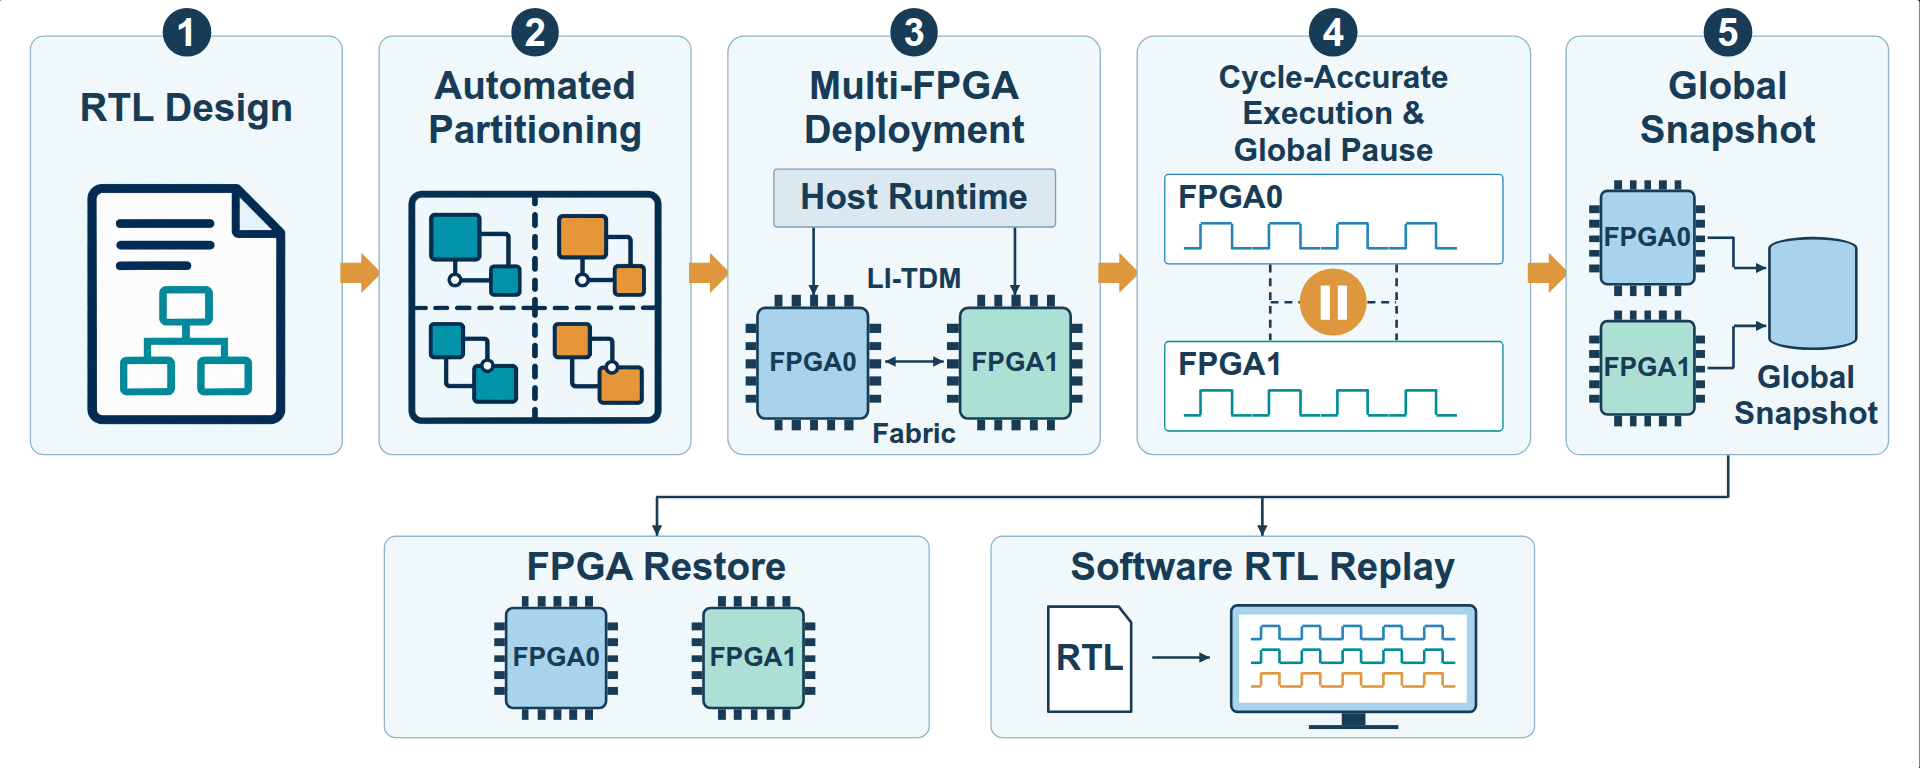
\includegraphics[width=\linewidth]{figure/fpga-rtl-workflow.png}
    \caption{REMUS总体技术路线示意图}
    \label{fig:remus-overall-workflow}
\end{figure}

\paragraph{中期阶段进展}

在自动化划分方面，已形成从层次化RTL分析、资源估计到超图划分和RTL子设计生成的处理流程。现阶段已完成自适应粒度处理、标量资源权重构建与KaHyPar求解，以及划分后组合路径的切割数分析和传播阶段参数配置。不同划分粒度的效果、标量均衡与实际资源分布的关系，以及划分结果对运行效率的影响，还需要通过对照实验进一步评价。

在周期精确执行方面，已搭建多分区Cosim环境，开展LI-TDM跨分区传播、逻辑周期推进及一致暂停的验证，并对传播阶段的首尾收发流程进行了优化。以PicoRV32和香山昆明湖（KMH）为对象的已有测试，已对照程序执行结果、暂停周期及部分内部状态，在所测试范围内得到一致结果。更长区间和更广内部状态范围的对照仍需完善。

分布式状态管理已在REMU原有扫描与重放功能上完成多分区扩展。各FPGA的局部扫描数据可以汇聚为全局检查点，并依据编译生成的状态映射与未划分DUT进行对照。已有PicoRV32和KMH的Cosim测试，在所选暂停点比较的内部状态范围内得到一致结果。此外，针对非零周期检查点，已开展软件RTL重放以及FPGA上的恢复与重放测试，后续执行结果和再次保存的检查点数据符合预期。

系统实现方面，已基于PCIe直连Runtime完成双FPGA原型系统集成，PicoRV32与Rocket运行裸机程序，Nanhu与单核KMH运行OpenSBI及Linux命令行。已归档PicoRV32和KMH的部分运行与检查点计时、五个设计的双分区综合资源，以及2、3、4分区的划分与扫描规模。Fabric组件与双节点Role联调环境也已建立，但完整联合验收和板级验证仍需继续；其结果不与PCIe直连平台混同。

\paragraph{下一阶段研究计划}

后续将重点补充功能正确性与性能评估：对于周期控制和状态管理，需要扩大暂停场景与状态比较范围，实现多周期bit精确的内部状态验证。对于自动划分，将在相同DUT和资源约束下对比不同划分算法、划分粒度，统计Cut Size、最大路径切割数、处理开销及综合后的资源占用，分析资源估计与实际结果之间的差异。

在系统层面，将继续完善多FPGA原型并扩展实验配置，测量跨分区通信、统一控制、检查点数据传输和端到端运行的开销。相关实验需要区分Cosim与实际FPGA平台的结果，以明确各项方法的适用条件和局限。最终研究结论将以补充完成的实验和对照数据为依据。

